\begin{lstlisting}
习题3.3第1,2,9题

习题3.4第1,2,3,4,7,13题
\end{lstlisting}
\begin{exercise}
\begin{figure}[H]
\centering
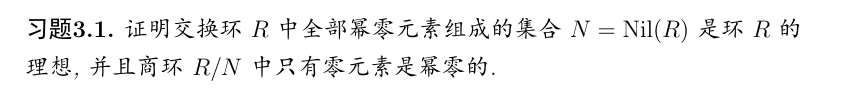
\includegraphics[width=\textwidth]{hw8-2025051020.png}
% \caption{}
\label{}
\end{figure}
\end{exercise}
\begin{proof}
$\forall a\in R,\forall n\in N$, $n^{m}=0$ for some $m\in \mathbb{N}$; then $(an)^{m}=a^{m}n^{m}=0$; thus $an\in N$. $\forall n_1, n_2\in N$, $n_1^{m_1}=n_2^{m_2}=0$ for some $m_1, m_2\in \mathbb{N}$; then $(n_1-n_2)^{m_1+m_2}=0$; thus $n_1-n_2\in N$. $N$ is an ideal in $R$.

Consider the quotient ring $R/N$; if $r+N$ is nilpotent, $(r+N)^{m}=r^{m}+N=0$ for some $m$; then $r^{m}\in N$; thus $r\in N$. $r+N=0$ in the quotient ring.
\end{proof}

\begin{exercise}
\begin{figure}[H]
\centering

\includegraphics[width=\textwidth]{1-hw8-2025051020.png}
% \caption{}
\label{}
\end{figure}
\end{exercise}
\begin{note}
$M_n(R)$ is the ring of $n \times n$ matrices with entries in the ring $R$.
\end{note}
\begin{proof}
Clearly, $M_n(I)$ is an ideal of the ring $M_n(R)$. Construct the ring homomorphisms
\[
\varphi:M_n(R)/M_n(I)\to M_n(R/I) \qquad (r_{ij})_{i,j}+M_n(I)\mapsto(r_{ij}+I)_{i,j}
\]
\[
\psi:M_n(R/I)\to M_n(R)/M_n(I)\qquad (r_{ij}+I)_{i,j}\mapsto(r_{ij})_{i,j}+M_n(I)
\]
Then $\varphi \circ \psi=id_{M_n(R/I)}$, $\psi \circ\varphi=id_{M_n(R)/M_n(I)}$. Thus
\[
M_n(R)/M_n(I)\cong M_n(R/I)
\]
\end{proof}

\begin{exercise}
\begin{figure}[H]
\centering
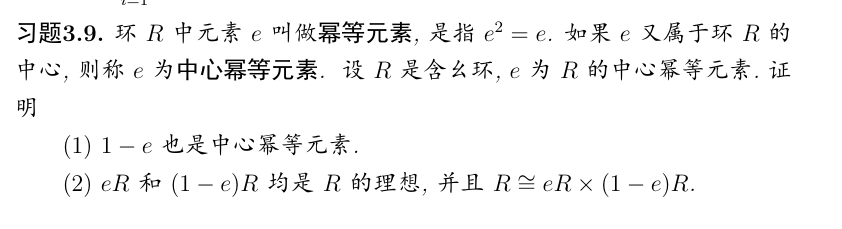
\includegraphics[width=\textwidth]{2-hw8-2025051020.png}
% \caption{}
\label{}
\end{figure}
\end{exercise}
\begin{proof}
(1)
The center of a ring $R$, denoted $Z(R)$, is defined as
\[
Z(R)=\{z \in R \mid zr=r z \text { for all } r \in R\}
\]
Since $er=re$ for any $r\in R$, then $(1-e)r=r-er=r-re=r(1-e)$; $1-e\in Z(R)$.

(2)
Check that $eR$ is an ideal in $R$.

For any $er\in eR$ and $a\in R$,
\[
a(er)=aer=e\underbrace{ ar }_{ \in R }\in eR
\]
For any $er_1, er_2\in eR$,
\[
er_1-er_2=e(\underbrace{ r_1-r_2 }_{ \in R })\in eR
\]
Thus $eR$ is an ideal in $R$. Similarly, $(1-e)R$ is an ideal in $R$.

Construct the mappings
\[
\varphi:R\to eR\times(1-e)R\qquad r\mapsto (er,(1-e)r)
\]
\[
\psi:eR\times(1-e)R\to R\qquad (er_1,(1-e)r_2)\mapsto er_1+(1-e)r_2
\]
We have
\[
\varphi(r+r')=(e(r+r'),(1-e)(r+r'))=(er,(1-e)r)+(er',(1-e)r')=\varphi(r)+\varphi(r')
\]
\[
\varphi(rr')=(err,(1-e)rr')
\]
\[
\begin{aligned}
\varphi(r)\varphi(r') & =(er,(1-e)r)\cdot(er',(1-e)r')=(er \cdot er',(1-e)r\cdot(1-e)r') \\
 & =(e^2rr',(1-e)^2rr')=(err',(1-e)rr')=\varphi(rr')
\end{aligned}
\]
\[
\varphi(1)=(e,1-e)
\]
\[
\psi((er_1,(1-e)r_2)+(er_1',(1-e)r_2'))=\psi(e(r_1+r_2),(1-e)(r_2+r_2'))=\psi(r_1)\psi(r_2)
\]
\[
\psi((er_1,(1-e)r_2)\cdot(er_1',(1-e)r_2'))=\psi(er_1r_1',(1-e)r_2r_2')=er_1r_1'+(1-e)r_2r_2'
\]
\[
\begin{aligned}
\psi(er_1,(1-e)r_2)\cdot \psi(er_1',(1-e)r_2') & =(er_1+(1-e)r_2)(er_1'+(1-e)r_2') \\
 & =er_1r_1'+\underbrace{ (1-e)e }_{ =0 }r_2r_1'+\underbrace{ e(1-e) }_{ =0 }r_1r_2'+(1-e)r_2r_2' \\
 & =er_1r_1'+(1-e)r_2r_2' \\
 & =\psi((er_1,(1-e)r_2)\cdot(er_1',(1-e)r_2'))
\end{aligned}
\]
\[
\psi(e,1-e)=1
\]
Thus $\varphi$ and $\psi$ are homomorphisms. Also $\varphi \circ \psi=id_{eR\times(1-e)R}$, $\psi \circ \varphi=id_{R}$. Then
\[
R\cong eR\times(1-e)R
\]
\end{proof}

\begin{exercise}
\begin{figure}[H]
\centering
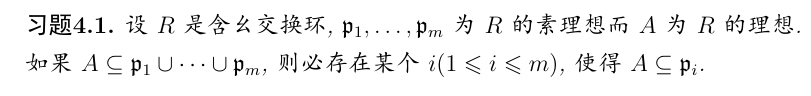
\includegraphics[width=\textwidth]{3-hw8-2025051020.png}
% \caption{}
\label{}
\end{figure}
\end{exercise}
\begin{proof}
We prove by induction on $n$ that
\begin{equation}
A\not\subseteq \mathfrak{p}_i\text{ for }i=1,\dots,n\implies A\not\subseteq \bigcup_{i=1}^{n} \mathfrak{p}_i
\label{0166c5}
\end{equation}

The base case $n=1$ is clear, and suppose that we have prove \cref{0166c5} for $n-1$, and now we prove this for $n$. By induction hypothesis, for each $i=1,\dots,n$, we may find $x_i\in $ such that
\[
x_i\not\in \mathfrak{p}_{1}\cup\dots \cup \mathfrak{p}_{i-1}\cup \mathfrak{p}_{i+1}\cup\dots \cup \mathfrak{p}_n
\]
If for some $x_i$, $x_i \not\in \mathfrak{p}_i$, we have already verified \cref{0166c5} using this element $x_i$. Now it suffices to treat the case when $x_i\in \mathfrak{p}_i$ for every $i=1,\dots,n$. Then consider the element
\[
y=\sum_{i=1}^{n} x_1\dots x_{i-1}x_{i+1}\dots x_n
\]
Clearly $y\in A$. We show that $y\not\in \mathfrak{p}_i$ for every $i$. Indeed, all elements in the sum except the $i$ th term $x_1\dots x_{i-1}x_{i+1}\dots x_n$ belongs to $\mathfrak{p}_i$. But as $\mathfrak{p}_i$ is a prime ideal, this product $x_1\dots x_{i-1}x_{i+1}\dots x_n$ does not belong to $\mathfrak{p}_i$. So $y\not\in \mathfrak{p}_i$. This completes the inductive proof.
\end{proof}

\begin{exercise}
\begin{figure}[H]
\centering

\includegraphics[width=\textwidth]{4-hw8-2025051020.png}
% \caption{}
\label{}
\end{figure}
\end{exercise}
\begin{proof}
Let $R$ be a finite commutative ring with prime ideal $\mathfrak{p}$. Then $R/\mathfrak{p}$ is an integral domain. As finite integral domain is field, $\mathfrak{p}$ is maximal in $R$.
\end{proof}
\begin{figure}[H]
\centering
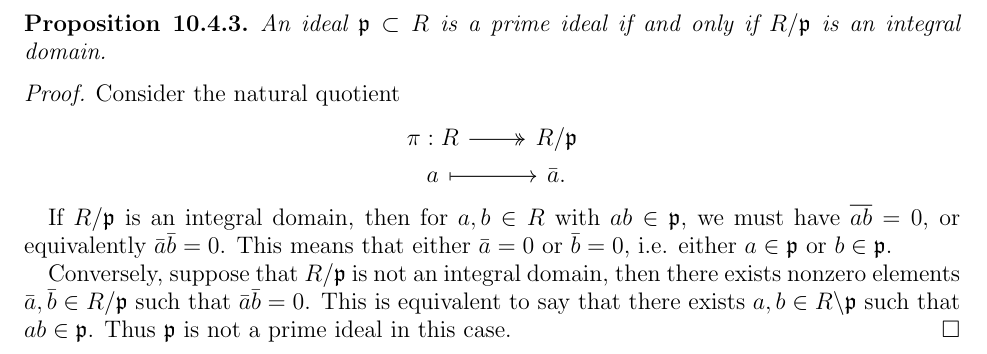
\includegraphics[width=\textwidth]{hw8-2025051100.png}
% \caption{}
\label{}
\end{figure}
\begin{figure}[H]
\centering
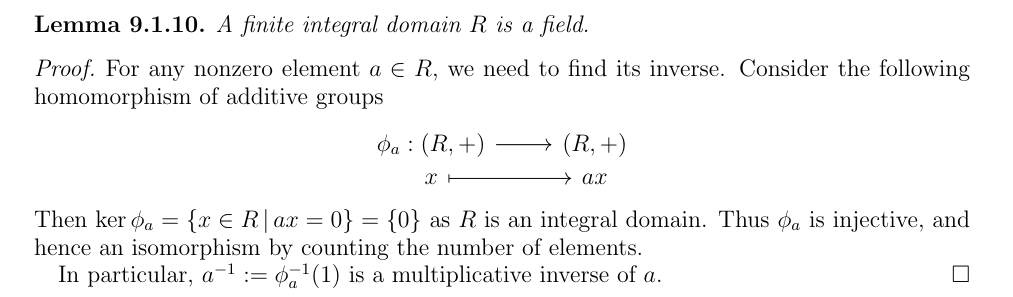
\includegraphics[width=\textwidth]{1-hw8-2025051100.png}
% \caption{}
\label{}
\end{figure}
\begin{figure}[H]
\centering
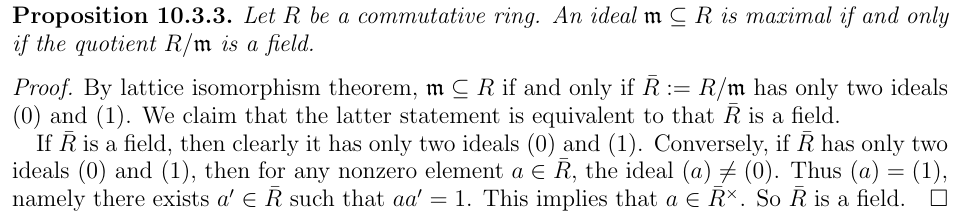
\includegraphics[width=\textwidth]{4-hw8-2025051100.png}
% \caption{}
\label{}
\end{figure}

\begin{exercise}
\begin{figure}[H]
\centering

\includegraphics[width=\textwidth]{5-hw8-2025051020.png}
% \caption{}
\label{}
\end{figure}
\end{exercise}
\begin{proof}
If $\mathrm{Nil}(R)\not \subseteq \mathfrak{p}$ for some $\mathfrak{p}$, pick $x\in \mathrm{Nil}(R)\setminus \mathfrak{p}$, then
\[
x\not\in \mathfrak{p}\Rightarrow x^2\not\in \mathfrak{p}\Rightarrow\dots\Rightarrow0\not\in \mathfrak{p}
\]
which is a contradiction.
\end{proof}

\begin{exercise}
\begin{figure}[H]
\centering
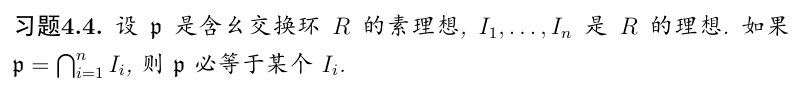
\includegraphics[width=\textwidth]{6-hw8-2025051020.png}
% \caption{}
\label{}
\end{figure}
\end{exercise}
\begin{proof}
$\mathfrak{p}\subseteq I_i$ for any $i=1,\dots,n$. Claim $I_i\subseteq \mathfrak{p}$ for some $i$. Assume not, pick $x_i\in I_i\setminus \mathfrak{p}$ for each $i$, then $y\coloneqq x_1\dots x_n\in I_i$ for each $i$; $y\in \mathfrak{p}$. But $x_i\not\in \mathfrak{p}$ for each $i$, as $\mathfrak{p}$ is prime, $y\not\in \mathfrak{p}$, which is a contradiction.
\end{proof}

\begin{exercise}
\begin{figure}[H]
\centering

\includegraphics[width=\textwidth]{7-hw8-2025051020.png}
% \caption{}
\label{}
\end{figure}
\end{exercise}
\begin{proof}
\[
\mathrm{Spec}(\mathbb{Z}/m\mathbb{Z})=\{ p\mathbb{Z}:\text{prime }p\mid m \}
\]
\[
\mathrm{Max}(\mathbb{Z}/m\mathbb{Z})=\left\{  \frac{m}{p}\mathbb{Z}:\text{prime }p\mid m  \right\}
\]
\end{proof}

\begin{figure}[H]
\centering
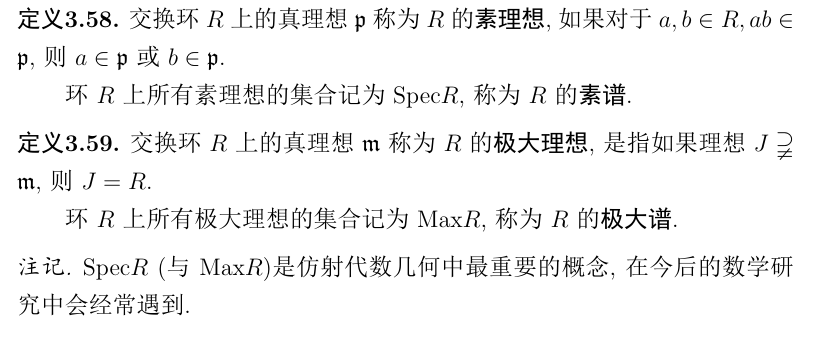
\includegraphics[width=\textwidth]{hw8-2025051101.png}
% \caption{}
\label{}
\end{figure}

\begin{exercise}
$R$ is PID; $F$ is its quotient domain; $S\supseteq R$ is subring of $F$. Show that $S$ is PID.
\end{exercise}
\begin{proof}
Let $I$ be an ideal in $S$, $J=I\cap R$. Then for any $x, y\in J$, $x-y\in I$ and $x-y\in R$, thus $x-y\in J$. For any $a\in R, x\in J$, $ax\in I$ and $ax\in R$, then $ax\in J$. $J$ is an ideal in $R$. As $R$ is PID, $J=(c)_{R}=cR$ for some $c$ in $R$.

Claim that $I=(c)_{S}=cS$. Clearly, $cS\subseteq I$. We need to show $I\subseteq cS$. For any $\frac{a}{b}\in I\subseteq S$, $a\in R$, $b\in R\setminus \{ 0 \}$. Since $F$ is fraction field over PID, WLOG, assume that $\gcd(a,b)=1$; i.e. $pa+qb=1$ for some $p, q\in R$. Then
\[
\underbrace{ \underbrace{ p }_{ \in R\subseteq S }\cdot\underbrace{ \frac{a}{b} }_{ \in S } }_{ \in S }+\underbrace{ q }_{ \in R\subseteq S }=\frac{1}{b}\implies \frac{1}{b}\in S
\]
Since $a=b\cdot\frac{a}{b}\in I$ and $a\in R$, we have $a\in J$ thus $a=kc$ for some $k\in R$. Then
\[
\frac{a}{b}=\frac{kc}{b}=c\cdot \underbrace{ k\cdot\frac{1}{b} }_{ \in S }\in cS
\]
Therefore $I=cS=(c)_{S}$. Hence $S$ is PID.

\end{proof}
